\section{Métodos inferiores}
Os quatro algoritmos classificados neste trabalho como inferiores possuem, como já detalhado em capítulos anteriores, complexidade temporal quadrática no tamanho do vetor de entrada. Eles recebem essa denominação por apresentarem, de acordo com a análise de complexidade apresentada no Capítulo \ref{cap:inferiores}, essa ordem de crescimento. Entretanto, embora todos apresentem a mesma complexidade assintótica, os testes práticos demonstraram que eles possuem desempenhos distintos.

Como o tempo de execução desses algoritmos apresenta crescimento quadrático à medida que o tamanho da entrada aumenta, o tamanho máximo do vetor utilizado foi $n=10^5$. Este tamanho foi considerado razoável para a observação dos resultados esperados, mantendo um tempo de execução viável para os testes.

\subsection{Tempo de execução}
O gráfico a seguir apresenta os resultados de tempo de execução obtidos ao se executar algoritmos de ordenação inferiores.

\begin{figure}[H]
\Caption{\label{fig:inferiores-tempo}Métodos inferiores – Tamanho × Tempo (em segundos).}
\centering
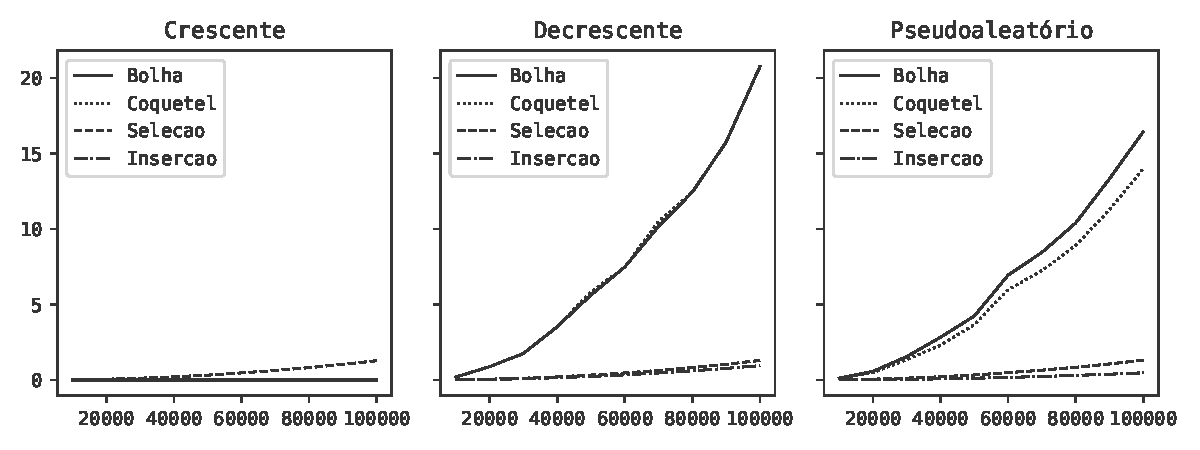
\includegraphics[scale=0.787]{figuras/pdf/inferiores.tempo.pdf}
\Fonte{Elaborado pelo autor}
\end{figure}

Para vetores já ordenados em ordem crescente, como esperado, apenas o algoritmo Selecao chegou a consumir mais de $1s$. Todos os demais algoritmos executaram apenas uma iteração e concluíram suas execuções, o que resultou em um tempo de consumo praticamente nulo.

O pior caso de todos os algoritmos fica evidente para vetores que, inicialmente, estão em ordem decrescente. Curiosamente, no entanto, os algoritmos Bolha e Coquetel se mostraram significativamente mais lentos que o Insercao e o Selecao. O motivo para esse desempenho será detalhado nas próximas seções, onde comparamos o número de comparações e movimentações que cada algoritmo realizou para este tipo de vetor.

Por fim, buscando observar o comportamento geral dos algoritmos, analisamos os vetores gerados de forma pseudoaleatória. Os algoritmos Bolha e Coquetel apresentaram uma leve melhora de desempenho, sendo o Coquetel ligeiramente mais rápido. Isso ocorre porque a iteração de retorno do Coquetel permite que elementos menores atinjam suas posições finais mais rapidamente do que no Bolha. Já os algoritmos Selecao e Insercao foram significativamente mais rápidos, com o Insercao apresentando o melhor resultado geral. Vale notar que o Selecao manteve praticamente o mesmo tempo de execução, independentemente do tipo de vetor. Tal fato se deve à sua característica de sempre executar uma quantidade fixa e quadrática de comparações, enquanto realiza um número mínimo de trocas. Dessa forma, o número de movimentações do Selecao é desprezível no tempo final de execução, o que o torna uma boa escolha para casos em que o vetor possui poucos elementos e a operação de movimentação tem um custo computacional elevado.


\subsection{Comparações}
O gráfico da Figura \ref{fig:inferiores-comparacoes} a seguir, exibe a relação entre o número de comparações e o tamanho do vetor para cada tipo de vetor analisado.

\begin{figure}[H]
\Caption{\label{fig:inferiores-comparacoes}Métodos inferiores – Tamanho × Comparações.}
\centering
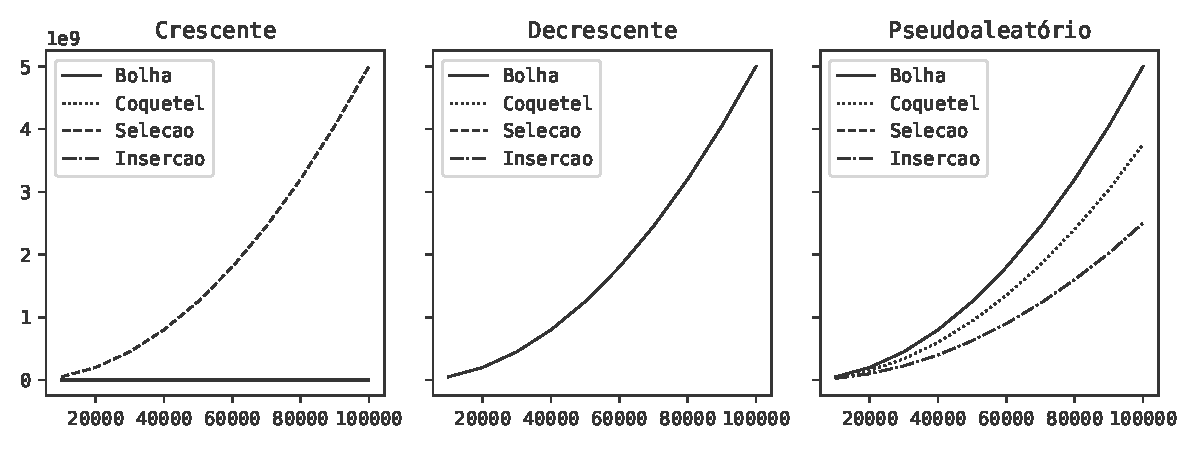
\includegraphics[scale=0.787]{figuras/pdf/inferiores.comparacoes.pdf}
\Fonte{Elaborado pelo autor}
\end{figure}

Para vetores em ordem crescente, como esperado, apenas o algoritmo Selecao executou uma quantidade quadrática de comparações. Os demais algoritmos, por outro lado, executaram uma quantidade linear de comparações, pois levaram apenas uma iteração externa para identificar que o vetor já se encontrava ordenado.

A análise teórica indicava que os algoritmos de ordenação inferiores apresentavam seu pior caso em comum: o vetor ordenado em ordem decrescente. Além disso, ela mostrava que esses algoritmos executam exatamente a mesma quantidade de comparações para esse tipo de vetor. Os testes práticos confirmaram essa conclusão, como é claramente demonstrado no gráfico.

No caso geral, com os vetores gerados de forma pseudoaleatória, pode-se observar que os algoritmos Bolha e Selecao permaneceram praticamente empatados em termos de número de comparações. O algoritmo Insercao demonstrou o melhor resultado, sendo aquele que necessitou do menor número de comparações para finalizar sua execução e garantir um vetor ordenado. Já o Coquetel ficou em um meio-termo, mostrando-se razoavelmente superior ao Bolha e ao Selecao nesse quesito. Sua vantagem reside no fato de que cada iteração externa coloca dois elementos em suas posições finais, além de aproximar os demais elementos de suas posições corretas em pelo menos uma posição.

\subsection{Movimentações}
O gráfico da Figura \ref{fig:inferiores-movimentacoes} a seguir, exibe a relação entre o número de movimentações e o tamanho do vetor para cada tipo de vetor analisado.

\begin{figure}[H]
\Caption{\label{fig:inferiores-movimentacoes}Métodos inferiores – Tamanho × Movimentações.}
\centering
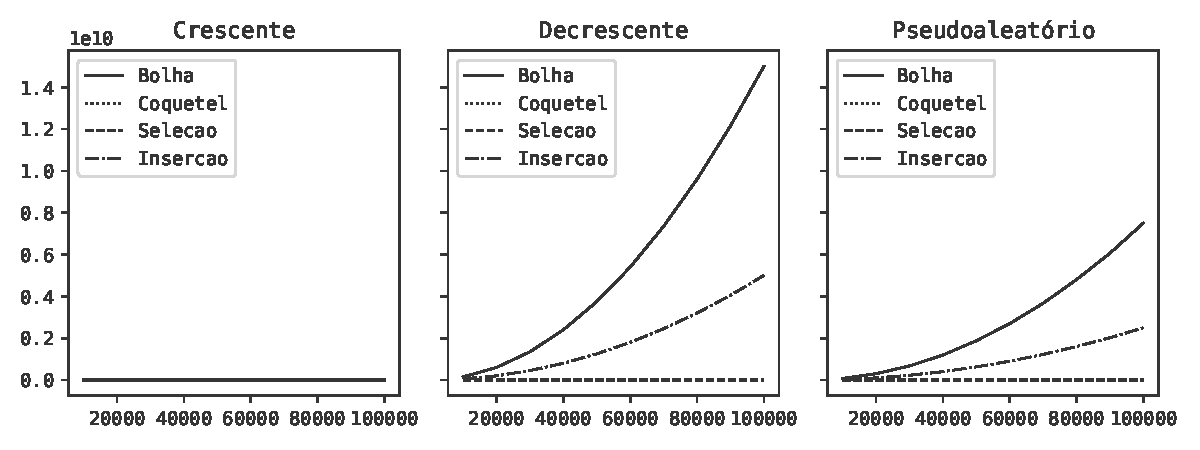
\includegraphics[scale=0.787]{figuras/pdf/inferiores.movimentacoes.pdf}
\Fonte{Elaborado pelo autor}
\end{figure}

Observe que, na prática, independentemente do tipo do vetor, os algoritmos Bolha e Coquetel possuem o mesmo desempenho com relação ao número de movimentações.

Neste ponto, pode-se estabelecer uma boa explicação para o Insercao ter apresentado o menor tempo de execução. Dentre todos os algoritmos inferiores, ele é o que melhor consegue equilibrar o número de comparações e movimentações. Ou seja, ele não possui extremos; enquanto o Bolha e o Coquetel geralmente executam muitas comparações e movimentações, e o Selecao executa muitas comparações e poucas movimentações, o Insercao permanece em um meio-termo. Essa característica o favorece, resultando em um tempo de execução menor que os demais para todos os tipos de vetores.

Quando o assunto é número de movimentações, o Selecao é o algoritmo mais eficiente. Isso ocorre porque ele executa sempre o número mínimo de trocas, garantindo que cada troca posicione pelo menos um elemento em sua posição definitiva. Dessa forma, ele realiza \bigO{n} movimentações, como fica evidente nos gráficos da Figura \ref{fig:selecao-movimentacoes} para todos os tipos de vetores. É importante notar que cada troca executa $3$ movimentações. Observe também que, para vetores decrescentes, cada troca posiciona dois elementos em suas posições finais.

\begin{figure}[H]
\Caption{\label{fig:selecao-movimentacoes}Selecao – Tamanho × Movimentações.}
\centering
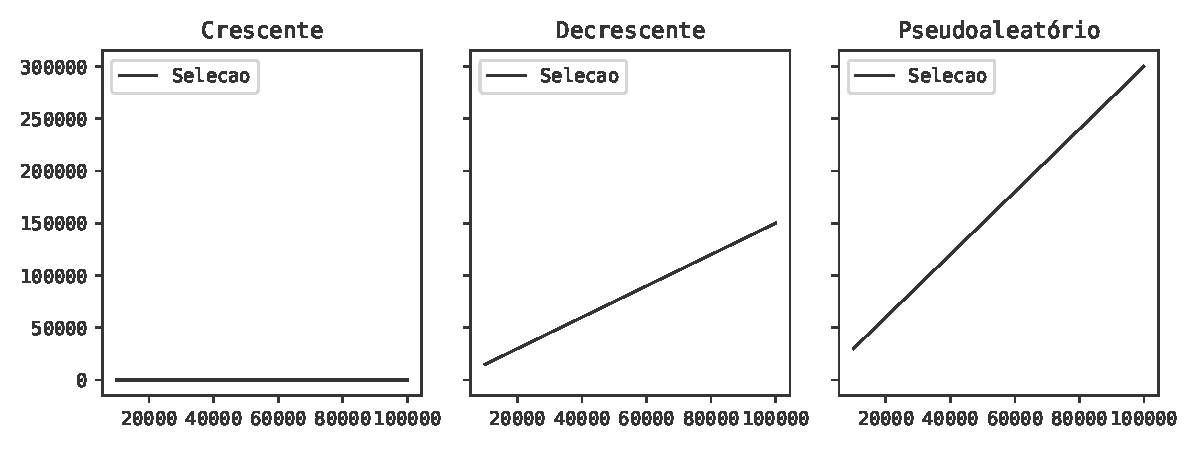
\includegraphics[scale=0.787]{figuras/pdf/selecao.movimentacoes.pdf}
\Fonte{Elaborado pelo autor}
\end{figure}
